\documentclass[border = 1cm, preview, varwidth = \maxdimen]{standalone}

\usepackage{xeCJK}
\usepackage{ifthen}

% mathematics
\usepackage{amsmath}
\usepackage{amssymb}
\usepackage{derivative}
\derivset{\pdif}[style-notation=multiple]
\usepackage{esint}

% tikz
\usepackage{tikz}
\usepackage{tikz-cd}
\usetikzlibrary{arrows}
\usetikzlibrary{automata}
\usetikzlibrary{positioning}
\tikzset{->, > = stealth', node distance = 2cm}
\tikzcdset{arrow style = tikz}

\begin{document}

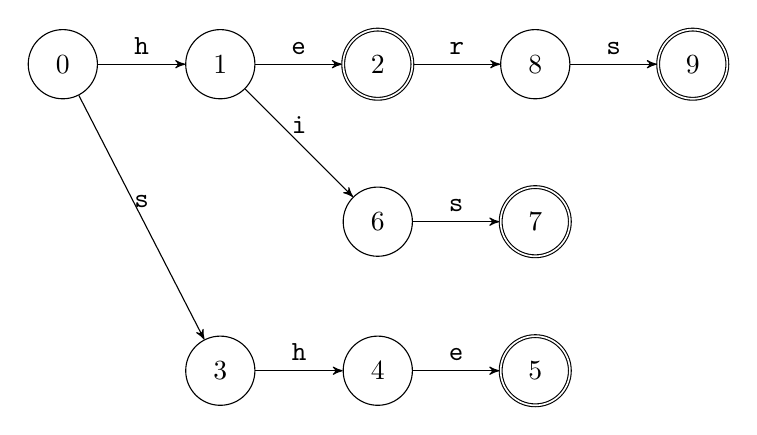
\begin{tikzpicture}
  % nodes
  \node (0) [state] {0};
  \node (1) [state, right of = 0] {1};
  \node (2) [state, accepting, right of = 1] {2};
  \node (3) [state, below = 3 of 1] {3};
  \node (4) [state, right of = 3] {4};
  \node (5) [state, accepting, right of = 4] {5};
  \node (6) [state, below of = 2] {6};
  \node (7) [state, accepting, right of = 6] {7};
  \node (8) [state, right of = 2] {8};
  \node (9) [state, accepting, right of = 8] {9};
  % edges
  \draw (0) edge [above] node {\tt h} (1);
  \draw (0) edge [above] node {\tt s} (3);
  \draw (1) edge [above] node {\tt e} (2);
  \draw (1) edge [above] node {\tt i} (6);
  \draw (2) edge [above] node {\tt r} (8);
  \draw (3) edge [above] node {\tt h} (4);
  \draw (4) edge [above] node {\tt e} (5);
  \draw (6) edge [above] node {\tt s} (7);
  \draw (8) edge [above] node {\tt s} (9);
\end{tikzpicture}

\end{document}

\iffalse
\[
  \begin{aligned}
    \int\frac{\mathrm dx}{x^3+1}&=\int\frac{\mathrm dx}{(x+1)\left(x^2-x+1\right)} \\
                                &=\frac16\int\frac2{x+1}-\frac{2x-1}{x^2-x+1}+\frac3{x^2-x+1}\mathrm dx \\
                                &=\frac13\int\frac{\mathrm dx}{x+1}-\frac16\int\frac{2x-1}{x^2-x+1}\mathrm dx+\frac12\int\frac{\mathrm dx}{x^2-x+1} \\
                                &=\frac13\ln|x+1|-\frac16\int\frac{\mathrm d(x^2-x+1)}{x^2-x+1}+\frac1{\sqrt3}\arctan\frac{2x-1}{\sqrt3}+C \\
                                &=\frac13\ln|x+1|-\frac16\ln\left|x^2-x+1\right|+\frac1{\sqrt3}\arctan\frac{2x-1}{\sqrt3}+C \\
  \end{aligned}
\]

\begin{tikzcd}
  Z \arrow[r, "f"] \arrow[d, "g"]                   & X \arrow[d, "i_1"] \arrow[rdd, bend left, "j_1"] & \\
  Y \arrow[r, "i_2"] \arrow[rrd, bend right, "j_2"] & X\sqcup_ZY \arrow[rd, dashed, "u"]               & \\
                                                    &                                                  & Q
\end{tikzcd}

\begin{tabular} {l | l}
  测地线方程 & $\displaystyle\frac{\mathrm d^2\gamma^\lambda}{\mathrm dt^2}+\Gamma_{\mu\nu}^\lambda\frac{\mathrm d\gamma^\mu}{\mathrm dt}\frac{\mathrm d\gamma^\nu}{\mathrm dt}=0$ \\
  \\
  斯托克斯方程 & $\displaystyle\int_\Omega\mathrm d\omega=\int_{\partial\Omega}\omega$ \\
  \\
  拉格朗日方程 & $\displaystyle\frac{\mathrm d}{\mathrm dx}\frac{\partial\mathcal L}{\partial\dot{\mathbf q}}-\frac{\partial\mathcal L}{\partial\mathbf q}=\mathbf0$ \\
  \\
  欧拉公式 & $\displaystyle\mathrm e^{\mathrm i\theta}=\cos\theta+\mathrm i\sin\theta$ \\
  \\
  高斯积分 & $\displaystyle\int_{-\infty}^\infty\mathrm e^{-x^2}\mathrm dx=\sqrt\pi$ \\
\end{tabular}

\[\int_\gamma A(x,y)\mathrm dx+B(x,y)\mathrm dy=0.\]
\fi

\end{document}
